
%(BEGIN_QUESTION)
% Copyright 2010, Tony R. Kuphaldt, released under the Creative Commons Attribution License (v 1.0)
% This means you may do almost anything with this work of mine, so long as you give me proper credit

En vannkjølt generator ved et kraftverk har to kilder til kjølevann, hver kilde utstyrt med en strømningsbryter som går tilbake til sin normalt åpne tilstand hvis vannstrømmen gjennom røret stopper.  Hvis en av vannkildene slutter å levere kjølevann til generatoren (uansett årsak), vil den strømningsbryteren deaktiveres og slå på varsellyset.  Dette er tilstrekkelig, siden generatoren fortsatt får tilstrekkelig kjøling fra bare én kilde.  Hvis begge vannkildene slutter å levere vann, vil imidlertid en "trip"-solenoid de-energiseres for å stanse generatoren før den overopphetes:

$$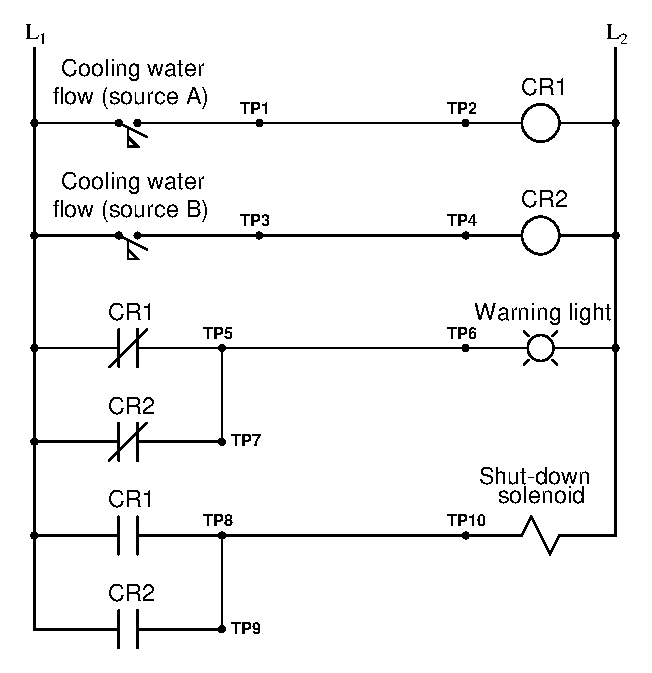
\includegraphics[width=15.5cm]{i00046x01.eps}$$

En dag stopper generatoren automatisk, selv om varsellyset aldri kom på.  En operatør verifiserer at det er tilstrekkelig kjølevannsstrøm gjennom begge rør.  Vurder sannsynligheten for hver spesifiserte feil i denne kretsen.  Vurder én feil om gangen (dvs. ingen samtidige feil), og avgjør om hver feil alene kan forklare {\it alle} symptomene i kretsen.

% No blank lines allowed between lines of an \halign structure!
% I use comments (%) instead, so that TeX doesn't choke.

$$\vbox{\offinterlineskip
\halign{\strut
\vrule \quad\hfil # \ \hfil & 
\vrule \quad\hfil # \ \hfil & 
\vrule \quad\hfil # \ \hfil \vrule \cr
\noalign{\hrule}
%
% First row
{\bf Feil} & {\bf Mulig} & {\bf Umulig} \cr
%
\noalign{\hrule}
%
% Another row
Solenoidspole feilet åpen &  &  \cr
%
\noalign{\hrule}
%
% Another row
Strømningsbryter A feilet åpen &  &  \cr
%
\noalign{\hrule}
%
% Another row
Strømningsbryter B feilet åpen &  &  \cr
%
\noalign{\hrule}
%
% Another row
Brudd i ledning TP5-TP6 &  &  \cr
%
\noalign{\hrule}
%
% Another row
Brudd i ledning TP8-TP9 &  &  \cr
%
\noalign{\hrule}
%
% Another row
Brudd i ledning TP8-TP10 &  &  \cr
%
\noalign{\hrule}
%
% Another row
Reléspole CR1 feilet åpen &  &  \cr
%
\noalign{\hrule}
%
% Another row
Reléspole CR2 feilet åpen &  &  \cr
%
\noalign{\hrule}
} % End of \halign 
}$$ % End of \vbox

Til slutt, identifiser den {\it neste} diagnostiske testen eller målingen du ville gjort på dette systemet.  Forklar hvordan resultatet/resultatene av denne testen eller målingen hjelper deg å identifisere plasseringen og/eller naturen til feilen.

\vfil 

\underbar{file i00046}
\eject
%(END_QUESTION)





%(BEGIN_ANSWER)

Dette er et vurdert spørsmål -- ingen svar eller hint gis!

%(END_ANSWER)





%(BEGIN_NOTES)

Vi ser av kretsanalysen at stoppsolenoiden er {\it de-energize to trip}.  Tilstrekkelig kjølevannsstrøm holder begge strømningsbrytere i aktivert (lukket) tilstand, og opprettholder dermed strøm til stoppsolenoiden via NO-relékontaktene.  Derfor kan vi konkludere med at solenoiden stanser generatoren ved {\it fravær} av påført strøm til den (dvs. hvis og når {\it begge} strømningsbrytere går til hviletilstand, som indikerer ingen kjølevannsstrøm).

\vskip 10pt

Basert på denne analysen, leter vi etter en feil som kan avbryte strømmen til stoppsolenoiden uten å påvirke varsellyset.  Dette begrenser feilsøket til et sted på den nederste rungen i skjemaet:

% No blank lines allowed between lines of an \halign structure!
% I use comments (%) instead, so that TeX doesn't choke.

$$\vbox{\offinterlineskip
\halign{\strut
\vrule \quad\hfil # \ \hfil & 
\vrule \quad\hfil # \ \hfil & 
\vrule \quad\hfil # \ \hfil \vrule \cr
\noalign{\hrule}
%
% First row
{\bf Feil} & {\bf Mulig} & {\bf Umulig} \cr
%
\noalign{\hrule}
%
% Another row
Solenoidspole feilet åpen & $\surd$ &  \cr
%
\noalign{\hrule}
%
% Another row
Strømningsbryter A feilet åpen &  & $\surd$ \cr
%
\noalign{\hrule}
%
% Another row
Strømningsbryter B feilet åpen &  & $\surd$ \cr
%
\noalign{\hrule}
%
% Another row
Brudd i ledning TP5-TP6 &  & $\surd$ \cr
%
\noalign{\hrule}
%
% Another row
Brudd i ledning TP8-TP9 &  & $\surd$ \cr
%
\noalign{\hrule}
%
% Another row
Brudd i ledning TP8-TP10 & $\surd$ &  \cr
%
\noalign{\hrule}
%
% Another row
Reléspole CR1 feilet åpen &  & $\surd$ \cr
%
\noalign{\hrule}
%
% Another row
Reléspole CR2 feilet åpen &  & $\surd$ \cr
%
\noalign{\hrule}
} % End of \halign 
}$$ % End of \vbox

En god "neste test" er å måle AC-spenning over solenoidspolen, for å se om den får strøm.  Hvis ja, er kablingen OK og det er solenoiden som har feilet.  Hvis nei, er kablingen årsaken til at solenoiden blir de-energiseret.


%INDEX% Switch, flow
%INDEX% Troubleshooting review: electric circuits

%(END_NOTES)
